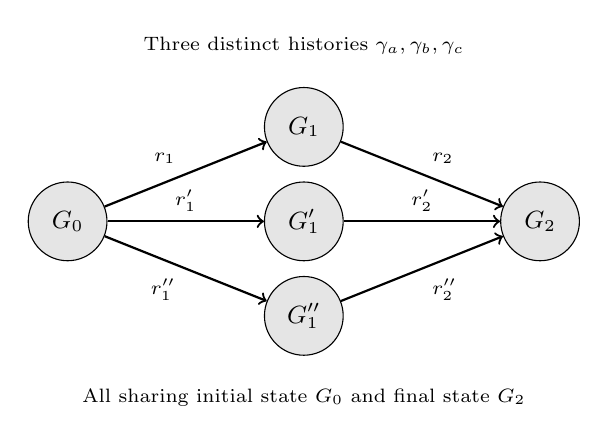
\begin{tikzpicture}[
    font=\small\sffamily,
    state/.style={circle, draw, fill=gray!20, minimum size=10mm, inner sep=0pt},
    history/.style={->, thick}
  ]

  % Initial state G_0
  \node[state] (g0) at (0,0) {$G_0$};

  % Multiple intermediate states
  \node[state] (g1a) at (3,1.2) {$G_1$};
  \node[state] (g1b) at (3,0) {$G_1'$};
  \node[state] (g1c) at (3,-1.2) {$G_1''$};

  % Final state G_2
  \node[state] (g2) at (6,0) {$G_2$};

  % Multiple paths from G_0 to intermediate states
  \draw[history] (g0) -- (g1a) node[midway, above left] {\scriptsize $r_1$};
  \draw[history] (g0) -- (g1b) node[midway, above] {\scriptsize $r_1'$};
  \draw[history] (g0) -- (g1c) node[midway, below left] {\scriptsize $r_1''$};

  % Multiple paths from intermediate states to G_2
  \draw[history] (g1a) -- (g2) node[midway, above right] {\scriptsize $r_2$};
  \draw[history] (g1b) -- (g2) node[midway, above] {\scriptsize $r_2'$};
  \draw[history] (g1c) -- (g2) node[midway, below right] {\scriptsize $r_2''$};

  % Labels for histories
  \node[align=center, font=\scriptsize, above] at (3, 2.0) {Three distinct histories $\gamma_a, \gamma_b, \gamma_c$};
  \node[align=center, font=\scriptsize, below] at (3, -2.0) {All sharing initial state $G_0$ and final state $G_2$};

\end{tikzpicture}
